% !TeX root = paper.tex


\chapter{車両タイプ判別モデルについて}
\section{この章で書くこと}
\begin{itemize}
	\item yoloとは
	\item 学習の実行
	\item 性能評価
	\item 作成したモデルの使い方
	\item 出力されるものについて
\end{itemize}

\section{YOLOとは}
YOLOの説明 \\
YOLOとはYou Only Look Onceの略で,人間のように一目見るだけで物体検出ができることを指している.データセットを作成し学習させることで,任意の物体のみ検出させることが可能である.\\
YOLOv8の説明   \\
YOLOv8はYOLOシリーズの最新バージョンであり,ディープラーニングとコンピュータビジョンの最先端の進歩に基づいており,速度と精度の麺で比類のない性能を提供している.
%https://docs.ultralytics.com/ja/ 参照

\section{学習の実行}
学習時にモデルの性能がそれまで以上に向上しなくなると学習が強制終了するため,エポック数という学習用データを何回繰り返して学習させるのかを表す数を10万回程度に設定して学習を進めた.強制終了した際のモデルが使用したデータセットで作れる最高の性能のモデルとなる.

\section{作成したモデルの使い方}
識別モデルと分類モデルで使い方はほとんど同じ
作成したモデルをロードして,モデルに画像または動画を渡すと識別または分類をすることができる\\
識別
\begin{verbatimx}
	$from ultralytics import YOLO
	model = YOLO("作成した識別モデルのパス")
	results = model.predict("画像のパス", save = True)
	$
\end{verbatimx}

分類
\begin{verbatimx}
	$from ultralytics import YOLO
	model = YOLO("作成した分類モデルのパス")
	results = model("画像のパス", save = True)
	$
\end{verbatimx}

\section{出力されるもの}
\begin{figure}	
	\centering
	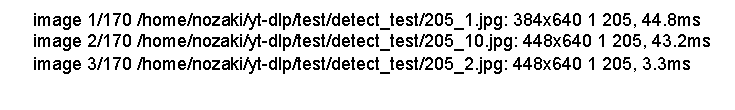
\includegraphics[width=\linewidth]{fig/a.pdf}
	\caption{出力されるもの}\label{output}
\end{figure}

\section{性能の評価}
\subsection{分類モデルの評価方法}
17種類の各車両の画像をそれぞれ10枚ずつ集めて画像の分類を行った.
分類モデルの予測した車両タイプと正解の車両タイプがどの程度あっているのか確かめることで性能の評価を行った.
\subsection{分類モデルの評価}
%分類モデルの評価を図\ref{CLS}に示す
\begin{figure}	
	\centering
	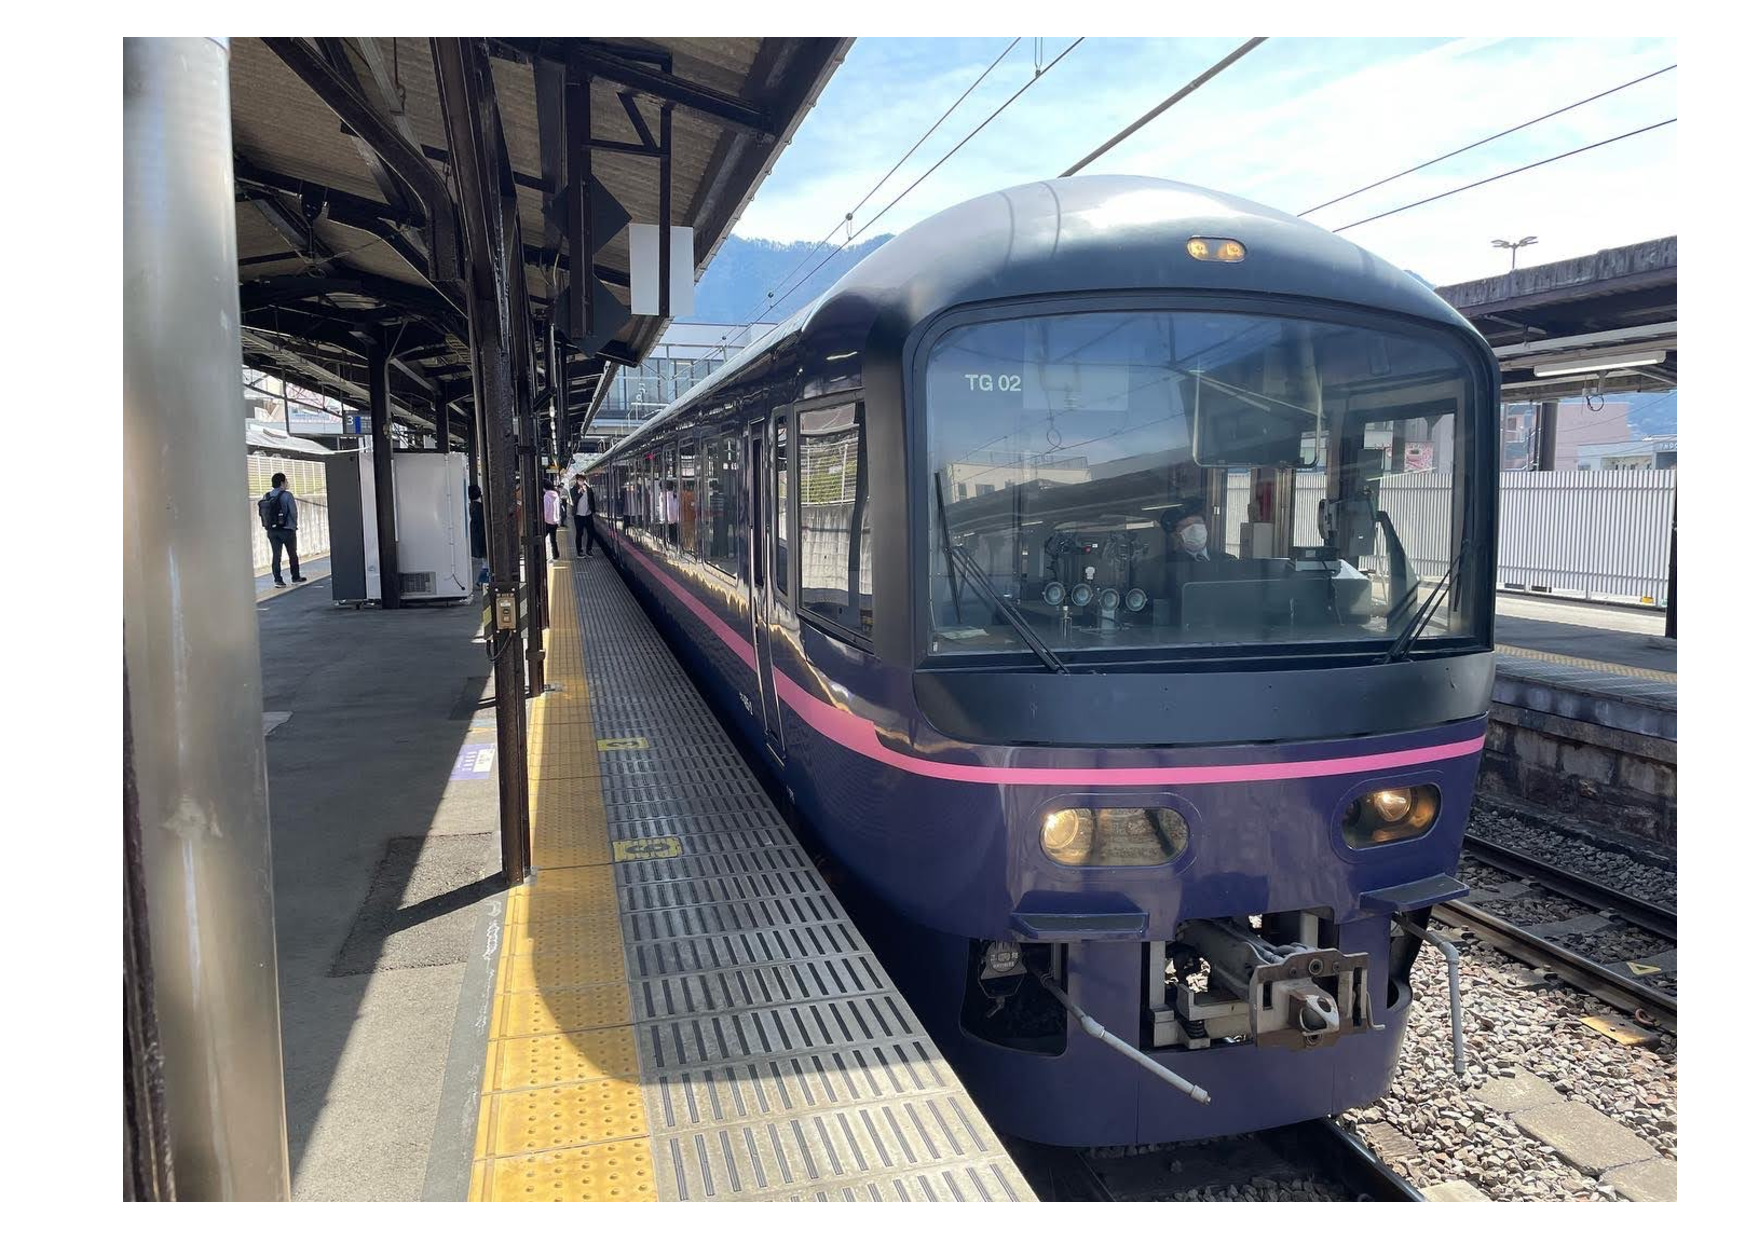
\includegraphics[width=\linewidth]{fig/hana.pdf}
	\caption{分類モデルの評価}\label{CLS}
\end{figure}
分類モデルの評価を図\ref{CLS}に示す.
縦軸が予測した車両タイプ,横軸が正解の車両タイプとするグラフである.
\subsection{識別モデルの評価方法}
%https://qiita.com/panchoooon/items/2c972ede2bc883597a87
作成したモデルは,IoUという指標で評価をする.
作成したモデルが車両タイプAだと認識した領域と車両タイプAの領域がどの程度重なっているのか,を表す指標である.
0.0 ≦ IoU ≦ 1.0の範囲で表され,IoUは1.0に近いほど正確に予測ができていることがわかる.
モデルが予測した領域と答えの領域が完全に一致しているときのIoUは1.0となり,全く重なりがない場合のIoUは0.0である.

\subsection{識別モデルの評価}
作成した識別モデルを使用し,テストデータセットの識別をした結果を表\ref{tab:identification_results} に示す.\\
NaNとは識別成功数または識別失敗数が0のときに,IoUの平均が出せない場合の値である.
\begin{table}[htbp] 
	\centering
	\begin{tabular}{cccccc}
		\hline
		車両タイプ & 識別成功数 & IoU(平均) & 識別失敗数 & IoU(平均) & 識別不能数 \\
		\hline \hline
		% ここにデータを入力
		\hline
		205 & 8 & 0.949791 & 1 & 0.913000 & 1 \\
		207 & 4 & 0.941828 & 2 & 0.940226 & 4 \\
		213 & 2 & 0.970088 & 7 & 0.923738 & 1 \\
		221 & 10 & 0.955405 & 0 & NaN & 0 \\
		223 & 8 & 0.970467 & 1 & 0.824151 & 1 \\
		225 & 1 & 0.688767 & 7 & 0.941395 & 2 \\
		227 & 4 & 0.953520 & 4 & 0.948728 & 2 \\
		271 & 5 & 0.844484 & 4 & 0.953993 & 1 \\
		281 & 2 & 0.838358 & 8 & 0.938570 & 0 \\
		283 & 7 & 0.953823 & 0 & NaN & 3 \\
		285 & 0 & NaN & 8 & 0.897906 & 2 \\
		287 & 5 & 0.960545 & 5 & 0.948412 & 0 \\
		321 & 8 & 0.932078 & 1 & 0.946316 & 1 \\
		323 & 9 & 0.954252 & 0 & NaN & 1 \\
		381 & 8 & 0.905294 & 1 & 0.950514 & 1 \\
		521 & 9 & 0.952872 & 1 & 0.810363 & 0 \\
		683 & 7 & 0.955607 & 3 & 0.962517 & 0 \\
		\hline
	\end{tabular}
	\caption{識別結果の表}
	\label{tab:identification_results}
\end{table}

